\chapter{Confidentialy}

A major aim of cryptography is to provide confidentiality. Any communication can be eavesdropped : cryptography ensures that the eavesdropper does not retrieve any important information from the raw communication datas.

This chapter will describe the major standard ciphers, from the one-time encryption through block cipher.

\section{One-Time Encryption}

The first family of the ciphers is the One-Time Ciphers : a cipher which use a unique key to encode a message. These ciphers are simple (yet unconvenient to use) and can reveal difficult to break (even impossible for the One-Time Pad). However, we will focus on the One-Time Pad, which is the most important one-time cipher. 

\section{One-Time Pad}

The One-Time Pad (OTP) is a symmetric cipher created for telegraph messages encryption and diplomatic communications during the beginning the twentieth century. It has been proved by Claude Shannon \footnote{Another computer science deity} to be theoretically secure. The OTP is fairly simple, yet powerful and has a lot of real-world applications (it is suggested that the OTP is used for the Washington-Moscow hotline during the Cold War).

\subsection{XOR operator}

The OTP is built from XOR operations. Since this operator has a lot of applications in cryptography, let revise it : the XOR operator is an "exclusive OR", in other words a and b can be true, but not both.


\begin{mydef}
\begin{minipage}[t]{0.8\textwidth}
\centering
    $XOR(a,b) = a \xor b = (a\&(\lnot b)) | ((\lnot a)\&b)$
\end{minipage}
\end{mydef}

\begin{table}[ht!]
	\centering
		\begin{tabular}{c|c|c}
			$A$ & $B$ & $A\xor B$ \\
			\hline
			0 & 0 & 0 \\
			0 & 1 & 1 \\
			1 & 0 & 1 \\
			1 & 1 & 0 \\
			\hline 
		\end{tabular}
	\caption{Table of logic for XOR}
	\label{tab:TableOfLogicForXOR}
\end{table}

\begin{mytheorem}
    $ a \xor a = False $
\end{mytheorem}
This corollary is really important since it's the key behind symmetric encryption using OTP.

\subsection{Cipher}

\begin{mydef}
\begin{minipage}[t]{0.8\textwidth}
	$ E(k,m) = c = k \xor m $ \\
	$ D(k,c ) = m = k \xor c$
\end{minipage}
\end{mydef}

An example of encryption :
\begin{align*}
    msg: & 0 1 1 0 1 1 1      \\
    key: & 1 0 1 1 0 1 0      \\
    cipher: & 1 1 0 1 1 0 1  \\
\end{align*}
To encrypt text-based datas, one must first use a character-encoding scheme (ASCII and  EBCDIC being the most well-known) to translate characters into integer values which will be XOR'd. \\

Encryption of "HELLO" using "XMCKL" as a key, and letter's position in the alphabet as an encoding scheme :
\begin{align*}
    msg: & H E L L O        \\
    msg (binary) : & 7 4 11 11 14 \\
    key: & X M C K L   \\
    key (binay) :& 23 12 2 10 11 \\
    cipher (binay): & 30 16 13 21 25  \\
    cipher (mod 26) : & 4 16 13 21 25 \\
    cipher :& E Q N V Z  \\
\end{align*}

\begin{mytheorem}
    $ D(k, E(k,m) ) = k \xor E(k,m) = k \xor k \xor m = m $
\end{mytheorem}

The decryption takes advantage of the fact that $k \xor k$ is null. On a side note, this $\xor$ property has another consequence : $ c \xor m = k $ (the message is nullified). Given the plaintext and the ciphertext, we can recover the key (which isn't really much a problem since the key is used only once for the OTP).

\subsection{Properties}

One-time Pad's main property is to be information-theoritically unbreakable \footnote{the proof is fairly easy since $P[E(k,m) == c] = 1$ is a constant.}. In others words, the attacker , given only the ciphertext, cannot recover the plaintext message even with unlimited computing power. In the case of the ciphertext EQNVZ computed before, we can see it's the encryption of HELLO using XMCKL as key, but also the encryption of LATER using TQURI as key : given only the ciphertext, the attacker cannot recover the plaintext message or the key, since several combinations are plausible.
	
\subsection{Drawbacks}

\subsubsection{Many-time pad}
The OTP is unfortunately vulnerable to many-times encryption : if an attacker recover several cyphertexts ${c_1,c_2,...,c_n}$ encoded with the same key $k$, he is able to recover several parts of plaintext message. The attacks consists of computing $c_x\xor c_y$ operations, nullifying the encrypting key to reveal $m_x\xor m_y$. Given the character encoding scheme, it is fairly easy to reveal significants parts of text. That's why the OTP is called "One-Time" : the key must change every time there is an encryption. 

\subsubsection{Symmetricality}
The symmetricality of the One-Time pad encryption enforce the fact that the key must be shared between the emettor and the receptor. It particulary annoying in the OTP case, since the key as to change every time there is an encryption, and since the key must be long (see below).

\subsubsection{Key length}
As a consequence from the Shannon perfect secrecy theorem, the OTP key must be at least as long as the message. It is quite a bother, since half of the communication bandwith is lost on key exchanges.

\subsubsection{Tampering}
The OTP is really weak against cyphertext tampering.

\subsection{Conclusion}

The One-Time pad is the first - and only - cipher which provides perfect secrecy, which makes him powerful but impractical since the key must be as long as the message. That's why stream ciphers (and later one block ciphers) were invented : to palliate the uneasiness of OTP's use, unfortunately at the secrecy's expense. Among actual standards of cryptography (apart from OTP), none has perfect secrecy. 

\section{ Stream Ciphers }

In order to be able to reuse the same key for several messages, two types of ciphers were created : stream ciphers and block ciphers. The stream ciphers operate on unknown length messages while block ciphers needs to known the message's size and slice it into block before encrypt it.\\
The nature of stream ciphers make them easy to use for radiocommunications \footnote{The Enigma machine is a stream cipher} : RC4 for WEP\footnote{WIFI Exchange Protocol}, A5/1 for GSM, E0 for Bluetooth, \dots Their small complexity make them also easier to port to hardware ASIC. However, there were also historically easier to break than block ciphers.\\
Stream ciphers aren't as popular as they were before compared to block ciphers, but there are not dead : there is a project called "eStream" which identify new modern and secure stream ciphers (Salsa20, Rabbit, ...). 

\section{WEP}

Let's focus on WEP since it's well known that this protocol is broken and unsecure.The WEP cipher is built upon the RC4 PRG  with the following seed : 
\begin{align}
     WEP(key,message) = RC4(IV,k) \xor m 
\end{align}

The IV (initial vector) component is a paquet counter : every time a paquet is sent (or received), the IV counter is incremented.

\subsection{RC4 implementation}

The RC4 is implemented as a 256-bytes permutation table (whose values a initialized using the key and the key-schedule algorithm) and two 1-bytes pointers. 

\begin{figure}[hb!]
    \centering
       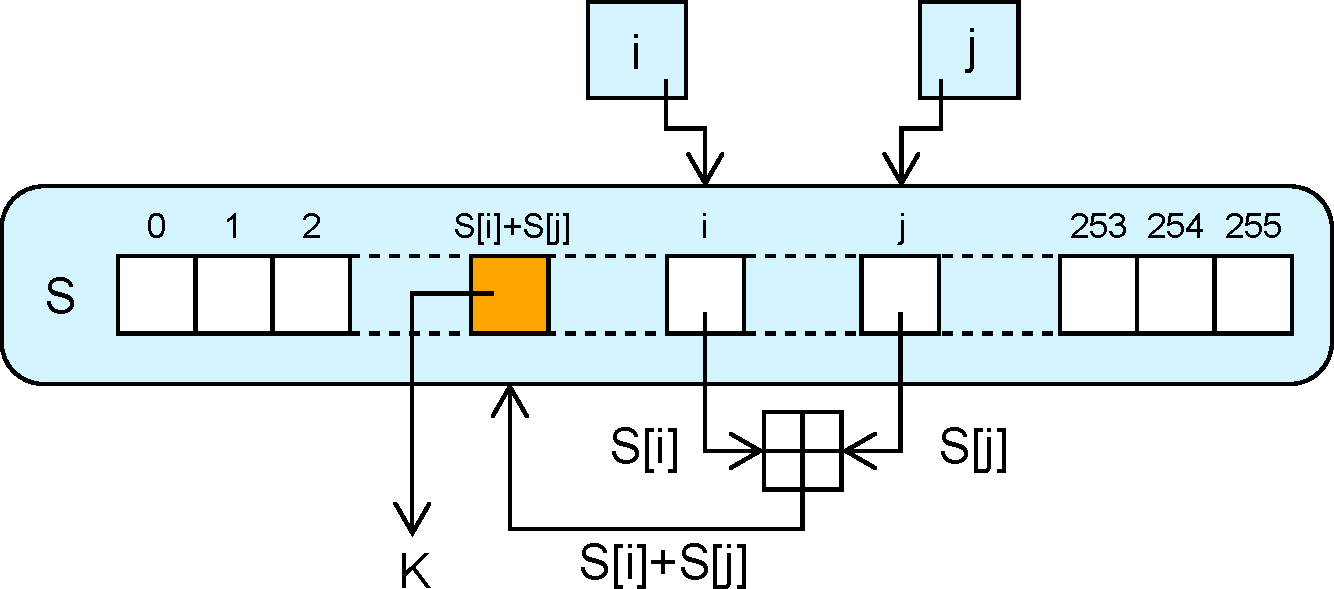
\includegraphics[width=\textwidth]{images/RC4.pdf}
	\caption{RC4 implementation \\ source : Wikipedia}
	\label{fig:RC4}
\end{figure}

Each cycle, i and j are incremented (modulo 256) and we perform the following operation : $k = S[ S[i] + S[j] \% 256$. Then we xor $k$ with the current message byte to obtain the ciphertext current byte.

\subsection{Vulnerabilities}
However, according to the  this IV is coded on 24 bits, which means it overflow every 16 millions of paquet cycle. 
It is a serious weakness, since we can use a two-time pad attack on paquet $0$ and paquet $2^24$ (which we know has the same IV and key). Moreover, at the initial handshake, the IV is fixed at 0 ! This fault completely break the WEP's security : by reseting the Access Point (AP) several times, it is fairly easy to recover the key (it is a matter of minutes).\\

\section{ Block Ciphers }


The block cipher has been created to be able to encode many message using the same key (thus reducing the number of key generated). In order to do so, the encryption has to be randomized (the random part sent along the cipherext)

\section{Data Encryption Standard (DES)}

The DES is a US standard created by the US. DOD \footnote{Department of Defense} in the 70's and built upon Feistel Networks as PRF. It has been broken by "exhaustive search" attacks in 1997 (and by others ways since).\\

\subsection{Feistel Network}

The backbone architecture behing DES is a 16-round Feistel cipher. The Feisel cipher has interesting properties and it's construct in the following manner : the input message (plaintext or ciphertext) is split in two parts $L_0$ and $R_0$ and feed through the structure. At each "round", an arbitrary function $f_i$ scramble the input message $L_i$ before xor'ing it with $R_i$.

\begin{figure}[ht!]
    \centering
       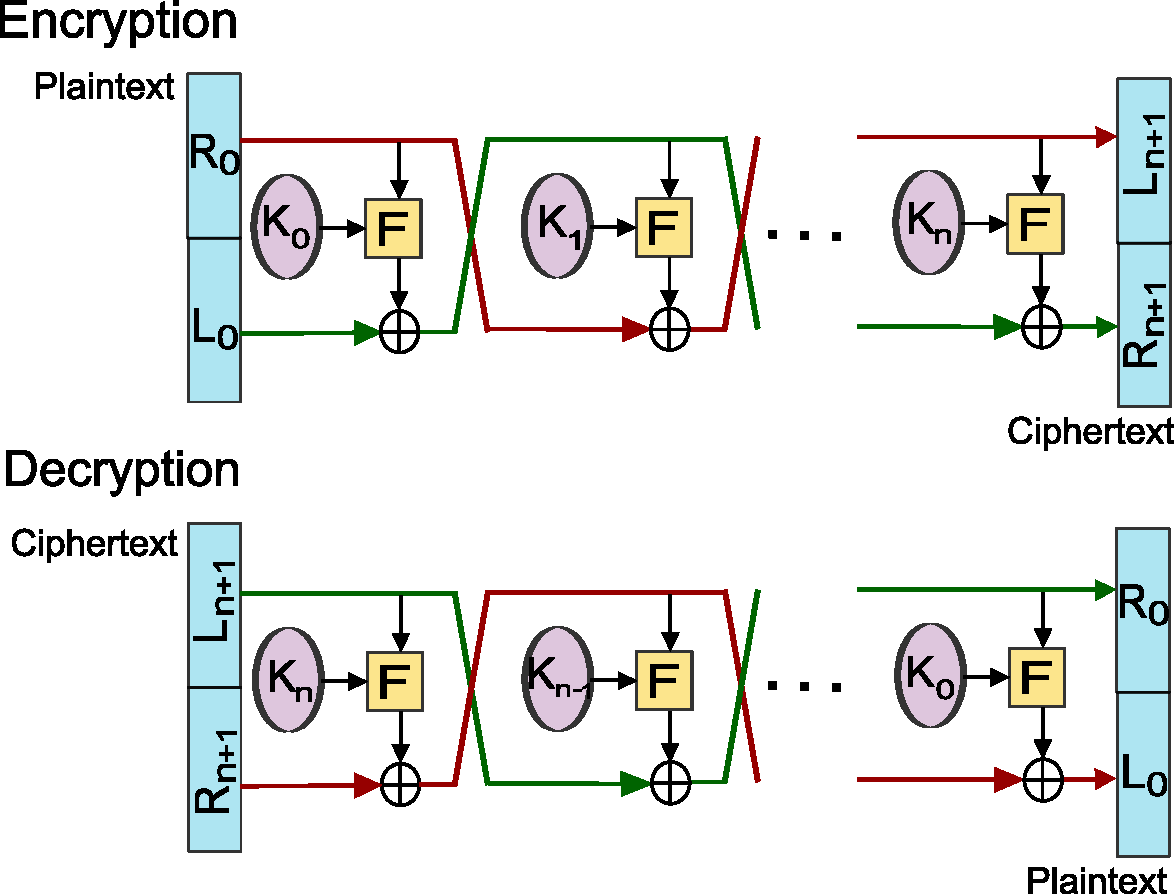
\includegraphics[width=\textwidth]{images/Feistel_cipher_encryption.pdf}
    \caption{Feistel cipher encryption and decryption \\ ( the arbitrary functions are generated using the secret key and a key-schedule. )\\ source : Wikipedia}
	\label{fig:Feistel_cipher}
\end{figure}
 

\begin{mytheorem}[Mathematical Formula]
    \begin{align}
        \forall i \in \llbracket1,m\rrbracket,&                 \\
        &L_i = R_{i-1}                                          \\
        &R_i = f_i(R_{i-1}) \xor L{i-1}                         
    \end{align}
\end{mytheorem}

The system is invertible, even if the arbitrary functions $f_i$ aren't : to decrypt a cyphertext, just invert the order the function to be applied. 
\begin{align}   
    \forall i \in \llbracket1,m\rrbracket,&                     \\
    &R_i = L_{i+1}                                              \\
    & L_i = f_{i+1}(L_{i+1}) \xor R{i+1}                    
\end{align}

This property is really handy since it halves the cipher's implementation in terms of space, electrical comsumption and parts prices.

\subsection{ DES construction }

The DES cipher works on 64-bit blocks encrypted by a 56-bit key, and it's constructed in the following manner : it has at first an initial permutation ($IP$), then a 16-round Feistel network with a key expansion alogrithm for the arbitrary functions, and finally the inverted initial permutation $IP^{-1}$ applied.

\subsubsection{Key schedule for DES}

The DES use a specific algroithm to expand the secret key into a family a subkey which will feed the Feistel family of PRF $f_0,f_1,\dots f_n$ : it is called a key schedule. Before decribing the key schedule, let's see the Feistel function f. 

Each PRF $f_i$ use a 48-bit subkey $k_i$ generated from the key-schedule and the 32-bit half-message from the previous round as input. The message is expanded to 48 bits to match the subkey's length, and the former is xor'ed with the latter.\\
The result is split in 6-bit value arrays (8 values if you can count). Each one of these 6-bit arrays goes through a 6-to-4 bits substitution functions $S_i$. For speed purposes, thoses $S_i$ boxes are often implemented as lookup-tables. \\
The result from the boxes is then recollected in a 32-bit message which goes through a final constant permutation function P in order to obtain the output. \\
The 56-bit key is expanded into sixteen 48-bit subkey using rotations and permutation ( see \cite{DES-wikipedia} ).

\begin{figure}[ht!]
    \centering
       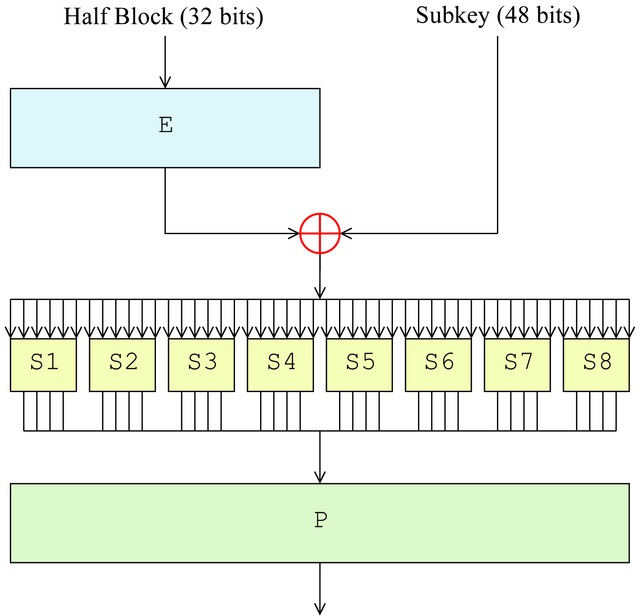
\includegraphics[width=0.7\textwidth]{images/DES-f-function.png}
    \caption{DES Festeil Function \\ source : Wikipedia}
	\label{fig:DES-f-function}
\end{figure}

\subsection{ Semantic security }

\begin{mytheorem}[Luby-Rackoff (1985)]
    Let $f:K\times\llbracket0,1\rrbracket^n -> \llbracket0,1\rrbracket^n$ a secure PRF, then the 3-round Feistel network is a secure PRP. \footnote{ you can see the proof here : \url{http://www.csc.kth.se/utbildning/kth/kurser/DD2448/krypto10/handouts/LR.pdf }}
\end{mytheorem}

The DES is a 16-round Feistel network, therefore it has the semantic security built on.  Even if the key schedule, S-boxes and initial permutation are known (they are fixed by the standard) it is not considered as a breach of security as long as the key remains unknown. The attacker may know the in and outs of the system, it should not be able to recover the plaintext message or the key.

\subsection{ Vulnerabilities }

The DES construction may be secure against cyphertext attacks in theory, it is not the case in reality. 

\subsection{DESx}

\section{Advanced Encryption Standard (AES)}

\subsection{Definition}

The AES cipher is the next generation of standard encryption, replacing DES. It has been created around 2000, and it currently widely use for symetric encryption (disk encryption with TrueCrypt, Wifi with WPA, ...). It exist two versions of the AES : the Cipher Block Chain (CBC) and the Randomized Counter Mode (CTR). 

\subsection{Cipher Block Chain construction (CBC)}

IV : intial vector (random).
$E_k : M -> C$ Encoder
$      m -> E(k,m)$

\subsubsection{Theorem}

$\forall L>0$, if E is a secure PRP over (K,X), then $E_{CBC}$ is a semantically secure cipher under CPA over $(K,X^L,X^{L+1})$.

$Adv_{CPA}[A,E_{CBC}] \leq 2.Adv_{PRP}[B,E] + 2.q^2.L^2/|X| $
q : nb of messages encrypted using key k
L : length of the message



\subsubsection{Construction with a Nonce-based IV}

\subsection{Randomized Counter Mode construction (CTR)}


\subsubsection{Theorem}

$\forall L>0$, if F is a secure PRF over (K,X), then $E_{CTR}$ is a semantically secure cipher under CPA over $(K,X^L,X^{L+1})$.

$Adv_{CPA}[A,E_{CTR}] \leq 2.Adv_{PRP}[B,F] + 2.q^2.L/|H| $
q : nb of messages encrypted using key k
H : length of the message

CTR construction is a bit better than CBC since the advantage is linear in the message's length (for CBC it is squared) and the algorithm is parralel (whereas it's sequential for CBC) which is easier to speed up (using FPGA or ASIC).
